\chapter{\MakeUppercase{Configuração do Estudo}}\label{sec:configuracao}

Este capítulo descreve como o estudo empírico foi planejado e executado, seguindo a estrutura recomendada por \citeonline{Wohlin2012} para experimentação em Engenharia de Software: definição das questões de pesquisa, coleta e preparação dos dados, operacionalização da ferramenta e protocolo de avaliação. A ordem das seções corresponde à ordem em que as etapas foram executadas, de modo que cada decisão de projeto possa ser rastreada até a questão de pesquisa que a motivou.

\section{Questões de Pesquisa}\label{sec2:rqs}

O objetivo geral do trabalho, construir uma ferramenta que prescreva quando e quanto vender do café colhido, foi decomposto em três questões de pesquisa. A primeira avalia o componente preditivo isoladamente; a segunda avalia o valor financeiro da prescrição; a terceira avalia a estabilidade da prescrição frente a variações nos parâmetros econômicos que o produtor não controla.

\begin{description}
	\item[RQ1 (Preditiva).] Em que medida uma rede LSTM alimentada por variáveis exógenas (preço do café robusta, taxa de câmbio, posição de fundos especulativos, clima nas regiões produtoras e preço de insumos) supera, em RMSE, MAE e MAPE, os métodos de referência disponíveis ao produtor na previsão do preço físico do café arábica nos horizontes de 21, 63 e 126 dias úteis após a colheita? Qual a contribuição de cada grupo de variáveis para essa acurácia?
	\item[RQ2 (Prescritiva).] Qual é o ganho financeiro líquido, medido em reais por saca em valor presente, obtido pela política de venda prescrita por programação dinâmica em comparação com as heurísticas usuais do produtor, descontados o custo mensal de armazenagem, a quebra técnica e o custo de oportunidade do capital à taxa Selic?
	\item[RQ3 (Robustez).] Quão sensível é a política ótima, em receita líquida e em frequência de decisões de armazenar, a variações na taxa Selic, no custo de armazenagem, no risco de base regional e no grau de aversão a risco do produtor?
\end{description}

A RQ1 difere de uma avaliação preditiva convencional em dois pontos. Primeiro, o alvo não é o preço em nível, mas o log-retorno futuro em cada horizonte, porque é essa grandeza que o motor de decisão consome. Segundo, os métodos de referência não se restringem ao passeio aleatório: inclui-se a curva de futuros da bolsa ICE ajustada pela base sazonal, que é a expectativa de preço que um produtor com acesso à B3 já possui sem nenhum modelo. Uma rede que não supere essa referência não agrega informação preditiva ao produtor, ainda que supere o passeio aleatório.

A RQ2 é a questão central do trabalho. Ela é respondida por \textit{backtesting} em safras fora da amostra de treino, sob a mesma contabilidade de custos para todas as estratégias comparadas. A RQ3 complementa a RQ2: uma política que só é lucrativa sob um conjunto estreito de parâmetros não é útil na prática, uma vez que Selic, tarifas de armazém e base regional variam de safra para safra e de cooperativa para cooperativa.

\section{Coleta de Dados}\label{sec2:coleta}

A coleta foi automatizada em módulos Python no pacote \texttt{src/data}, um por fonte, com a exceção do indicador CEPEA/ESALQ, cujo portal bloqueia requisições automatizadas e exige o download manual das planilhas. O \autoref{qua:fontes} resume as fontes efetivamente usadas na versão final, o papel de cada uma e as fontes descartadas ou substituídas ao longo do projeto.

\begin{quadro}[htb]
	\centering
	\caption{Fontes de dados da versão final do AgroVisible.}\label{qua:fontes}
	\begin{tabular}{L{3.6cm} L{3.4cm} L{5.2cm} L{2.2cm}}
		\hline
		\textbf{Dado} & \textbf{Fonte} & \textbf{Forma de coleta} & \textbf{Papel} \\ \hline
		Preço físico arábica e robusta (R\$/sc) & CEPEA/ESALQ & Planilhas XLS baixadas manualmente; leitura tolerante a arquivos corrompidos & Alvo e \textit{feature} \\
		Futuro \textit{Coffee C} (ICE NY) & Yahoo Finance (KC=F) & Série contínua do primeiro vencimento; curva por vencimento acumulada a partir de setembro de 2026 & \textit{Feature} e \textit{hedge} \\
		Câmbio PTAX e meta Selic & Banco Central, SGS (séries 1 e 432) & Biblioteca \texttt{python-bcb} & \textit{Feature} e custo de oportunidade \\
		Clima nas regiões produtoras & Open-Meteo (reanálise ERA5) & Temperatura mínima e precipitação diárias em Varginha, Patrocínio, Franca e Colatina & 5 \textit{features} \\
		Posição de fundos (COT) & CFTC & Biblioteca \texttt{cot-reports}, ancorada na data de divulgação & 2 \textit{features} \\
		Insumos (ureia, petróleo) & Banco Mundial, \textit{Pink Sheet} & Mensal, ancorado 3 dias úteis após o fechamento do mês & 3 \textit{features} \\
		Custos de produção (COE, COT, CT) & CONAB, série histórica & Planilha XLS por praça e ano; Guaxupé, MG & Motor: piso e margem \\ \hline
		Câmbio BRL=X (Yahoo) & --- & Descartado; substituído pela PTAX oficial & --- \\
		Robusta de Londres (RC=F) & --- & Contrato deslistado; substituído pelo indicador físico CEPEA do robusta & --- \\
		Estações INMET & --- & Descartado por cobertura irregular e lacunas por estação & --- \\ \hline
	\end{tabular}
	\fonte{Do autor (2026).}
\end{quadro}

Três escolhas de coleta merecem justificativa. A primeira é o uso do indicador CEPEA/ESALQ do café arábica tipo 6, bebida dura, como preço de venda do produtor. Não existe série pública de preço de balcão por cooperativa; o indicador é a média dos negócios nas praças de Minas Gerais e São Paulo e é a referência usada pelas próprias cooperativas na formação de seus preços. A segunda é a substituição do contrato de robusta de Londres pelo indicador físico do robusta no Brasil, imposta pela deslistagem do ticker na fonte de dados. A terceira é a preferência pela reanálise ERA5 em vez das estações do INMET: as estações apresentam lacunas de meses inteiros em várias localidades, o que impediria a construção de acumulados de chuva contínuos ao longo de duas décadas.

Os custos de produção vêm da série histórica de custos de produção do café arábica da CONAB, planilha de Guaxupé, Minas Gerais (agricultura familiar, cultivo semiadensado, alta tecnologia, semimecanizado). Dela são extraídos, por ano-safra, o custo variável, correspondente ao COE, o custo operacional, correspondente ao COT, e o custo total, todos em reais por saca. Os valores de COE para as safras de 2022 a 2025 são 766, 714, 784 e 876 R\$/sc. Durante o desenvolvimento foi usado um valor provisório de 700 R\$/sc, que se mostrou dentro da faixa.

\section{Engenharia de Dados}\label{sec2:pipeline}

\subsection{Alinhamento temporal}

As fontes têm calendários distintos: o indicador CEPEA é publicado em dias úteis brasileiros; a bolsa ICE segue o calendário norte-americano; o relatório COT é semanal; os preços de insumos são mensais; o clima é diário no calendário civil. O calendário-mestre adotado é o conjunto de dias em que existe indicador CEPEA publicado. As demais séries são projetadas sobre esse calendário com preenchimento pelo último valor conhecido (\textit{forward fill}), nunca por interpolação, que usaria valores ainda não observados.

Duas fontes exigiram cuidado adicional para evitar vazamento de informação futura. O relatório COT refere-se à posição de terça-feira, mas só é divulgado na sexta; as \textit{features} derivadas dele foram ancoradas na data de divulgação. Os preços mensais de insumos do Banco Mundial só ficam disponíveis alguns dias após o fechamento do mês; foram ancorados três dias úteis após o fim do mês de referência. Os acumulados de chuva foram calculados no calendário civil, antes do recorte para dias úteis, para que fins de semana e feriados chuvosos não fossem perdidos.

A base resultante cobre de 7 de dezembro de 2005 a 31 de agosto de 2026, com 5\,169 observações diárias e 45 colunas, sem valores faltantes. A série bruta do robusta começa em novembro de 2001, mas as médias móveis de dois anos e os retornos de um ano dos insumos consomem os quatro primeiros anos.

\subsection{Construção das variáveis de entrada}

A rede recebe 26 variáveis, todas construídas para serem estacionárias ou limitadas, organizadas em seis grupos: retornos, posição do preço em relação a médias móveis, mercado, calendário e macroeconomia, clima, fundos e insumos. O \autoref{qua:features} lista cada variável e sua definição.

\begin{quadro}[htb]
	\centering
	\caption{Variáveis de entrada da rede LSTM.}\label{qua:features}
	\begin{tabular}{L{2.4cm} L{4.2cm} L{7.8cm}}
		\hline
		\textbf{Grupo} & \textbf{Variável} & \textbf{Definição} \\ \hline
		Retornos & \texttt{ret\_arabica\_1d}, \texttt{ret\_arabica\_21d} & Log-retorno do físico arábica em 1 e 21 dias úteis \\
		& \texttt{ret\_robusta\_1d} & Log-retorno diário do físico robusta \\
		& \texttt{ret\_ice\_1d} & Log-retorno diário do futuro ICE \\
		& \texttt{ret\_ptax\_1d} & Log-retorno diário da PTAX \\
		Posição vs. média & \texttt{preco\_vs\_ma\_1m}, \texttt{\_3m}, \texttt{\_1a}, \texttt{\_2a} & Preço dividido pela média móvel de 21, 63, 252 e 504 dias, menos um \\
		Mercado & \texttt{vol\_21d} & Desvio-padrão anualizado dos retornos diários em 21 dias \\
		& \texttt{spread\_arabica\_robusta} & Razão entre os físicos arábica e robusta \\
		& \texttt{base\_fisico\_futuro\_pct} & (Físico $-$ ICE em R\$/sc) / ICE em R\$/sc \\
		Calendário e macro & \texttt{mes\_sin}, \texttt{mes\_cos} & Codificação cíclica do mês \\
		& \texttt{bienalidade\_alta} & Indicador de ano-safra de carga cheia (anos pares) \\
		& \texttt{selic\_meta} & Meta Selic, \% a.a. \\
		Clima & \texttt{chuva\_arabica\_30d}, \texttt{chuva\_arabica\_90d} & Chuva acumulada, média de Sul de Minas, Cerrado e Mogiana \\
		& \texttt{tmin\_arabica\_7d} & Mínima das temperaturas mínimas em 7 dias nas três regiões \\
		& \texttt{geada\_30d} & Indicador de $T_{\min} < 3\,^{\circ}$C entre maio e setembro nos últimos 30 dias. Constante igual a zero em toda a série: a reanálise não registra mínima abaixo de 3\,$^{\circ}$C em nenhum dos quatro pontos. Mantida como entrada inerte (ver \autoref{sec3:eda}) \\
		& \texttt{chuva\_robusta\_90d} & Chuva acumulada em Colatina, ES \\
		Fundos & \texttt{cot\_net\_pct\_oi} & Posição líquida não comercial sobre o \textit{open interest} \\
		& \texttt{cot\_net\_pct\_oi\_chg4w} & Variação da anterior em 20 dias úteis \\
		Insumos & \texttt{indice\_troca\_urea} & Sacas de café necessárias para comprar uma tonelada de ureia \\
		& \texttt{ret\_urea\_1a}, \texttt{ret\_crude\_1a} & Log-retorno de 252 dias da ureia e do petróleo \\ \hline
	\end{tabular}
	\fonte{Do autor (2026).}
\end{quadro}

Não há defasagens explícitas além das que a janela de entrada de 63 dias úteis fornece; a dependência temporal de prazo mais longo aparece como retornos acumulados e razões com médias móveis. A bienalidade da cultura é codificada como indicador binário do ano-safra de carga cheia, definido como o ano-safra que começa em julho de ano par.

\subsection{Análise exploratória das variáveis}\label{sec3:eda}

Antes do treinamento, cada variável foi confrontada com o alvo de cada horizonte no conjunto de treino por correlação de Spearman, e as variáveis foram confrontadas entre si para identificar colinearidade. A correlação de postos foi preferida à de Pearson porque as relações esperadas não são lineares e a estatística é robusta a valores extremos, frequentes em retornos. A \autoref{fig:corr-alvo} apresenta a correlação com o alvo por horizonte e a \autoref{fig:matriz-corr} a matriz entre variáveis.

\begin{figure}[htb]
	\centering
	\caption{Correlação de Spearman entre cada variável de entrada e o log-retorno futuro em 21, 63 e 126 dias úteis, no conjunto de treino.}\label{fig:corr-alvo}
	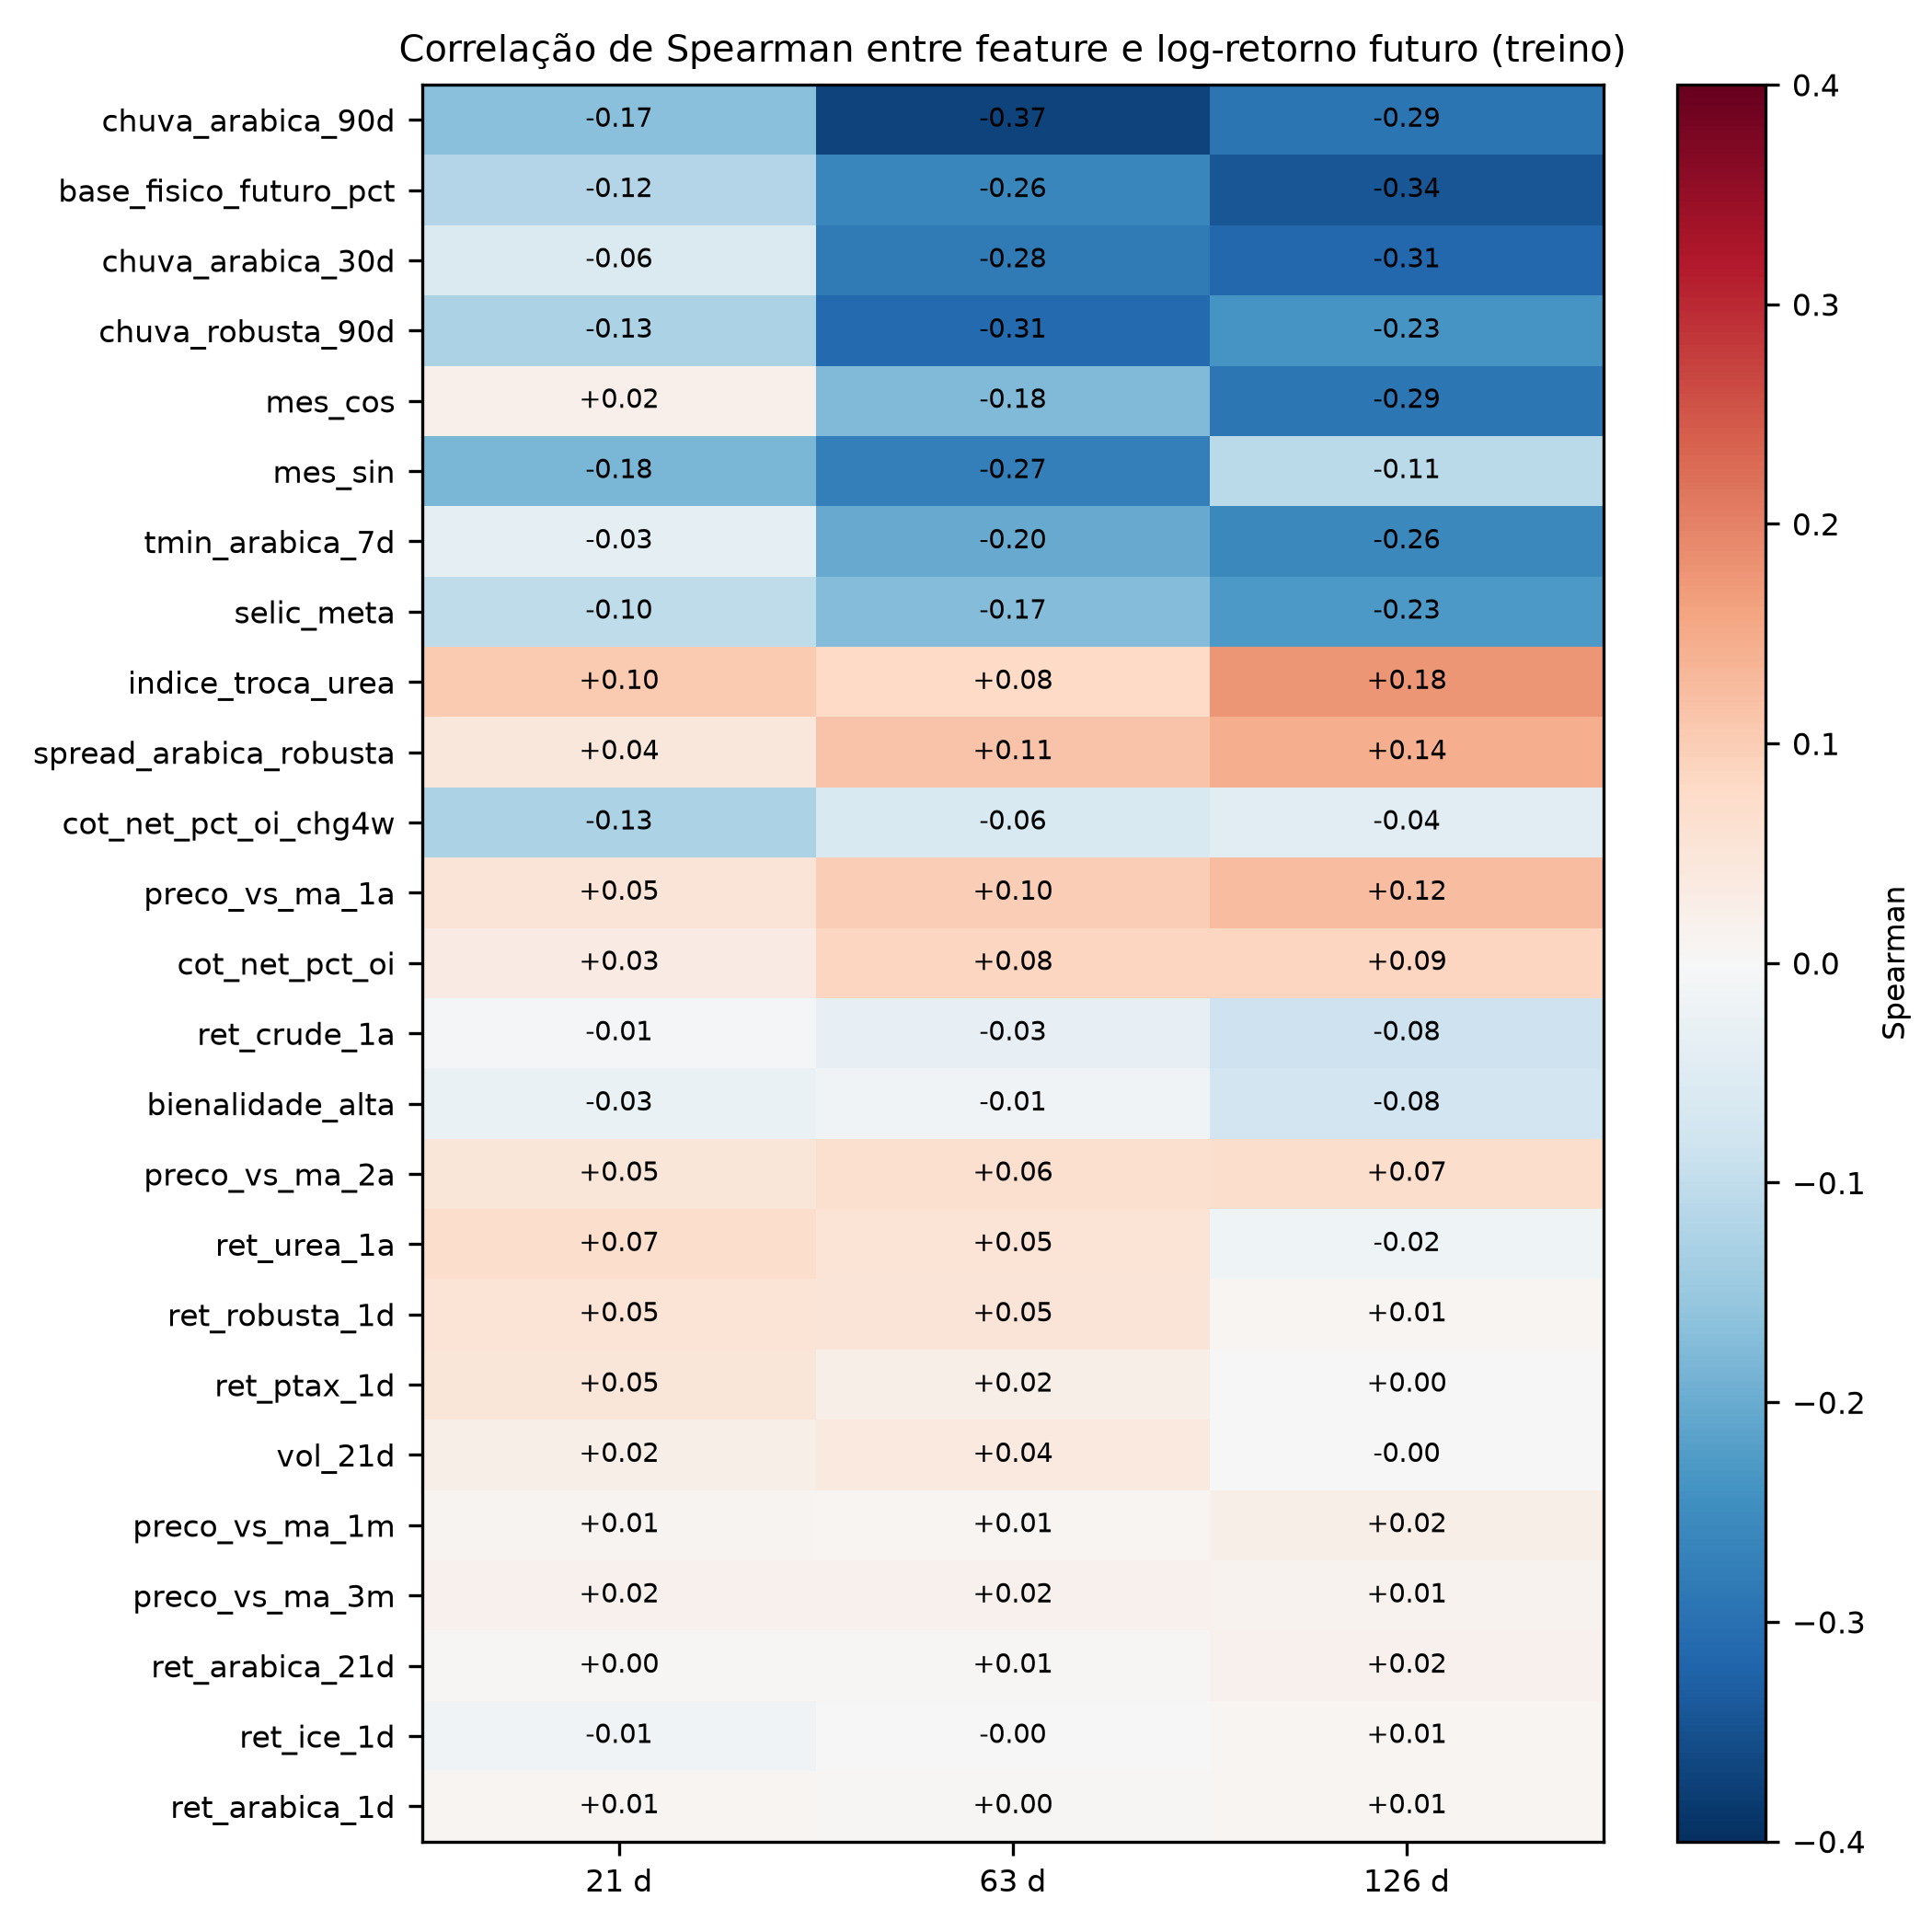
\includegraphics[width=0.95\textwidth]{imgs/10_corr_features_alvo.png}
	\fonte{Do autor (2026).}
\end{figure}

\begin{figure}[htb]
	\centering
	\caption{Matriz de correlação de Spearman entre as variáveis de entrada, no conjunto de treino.}\label{fig:matriz-corr}
	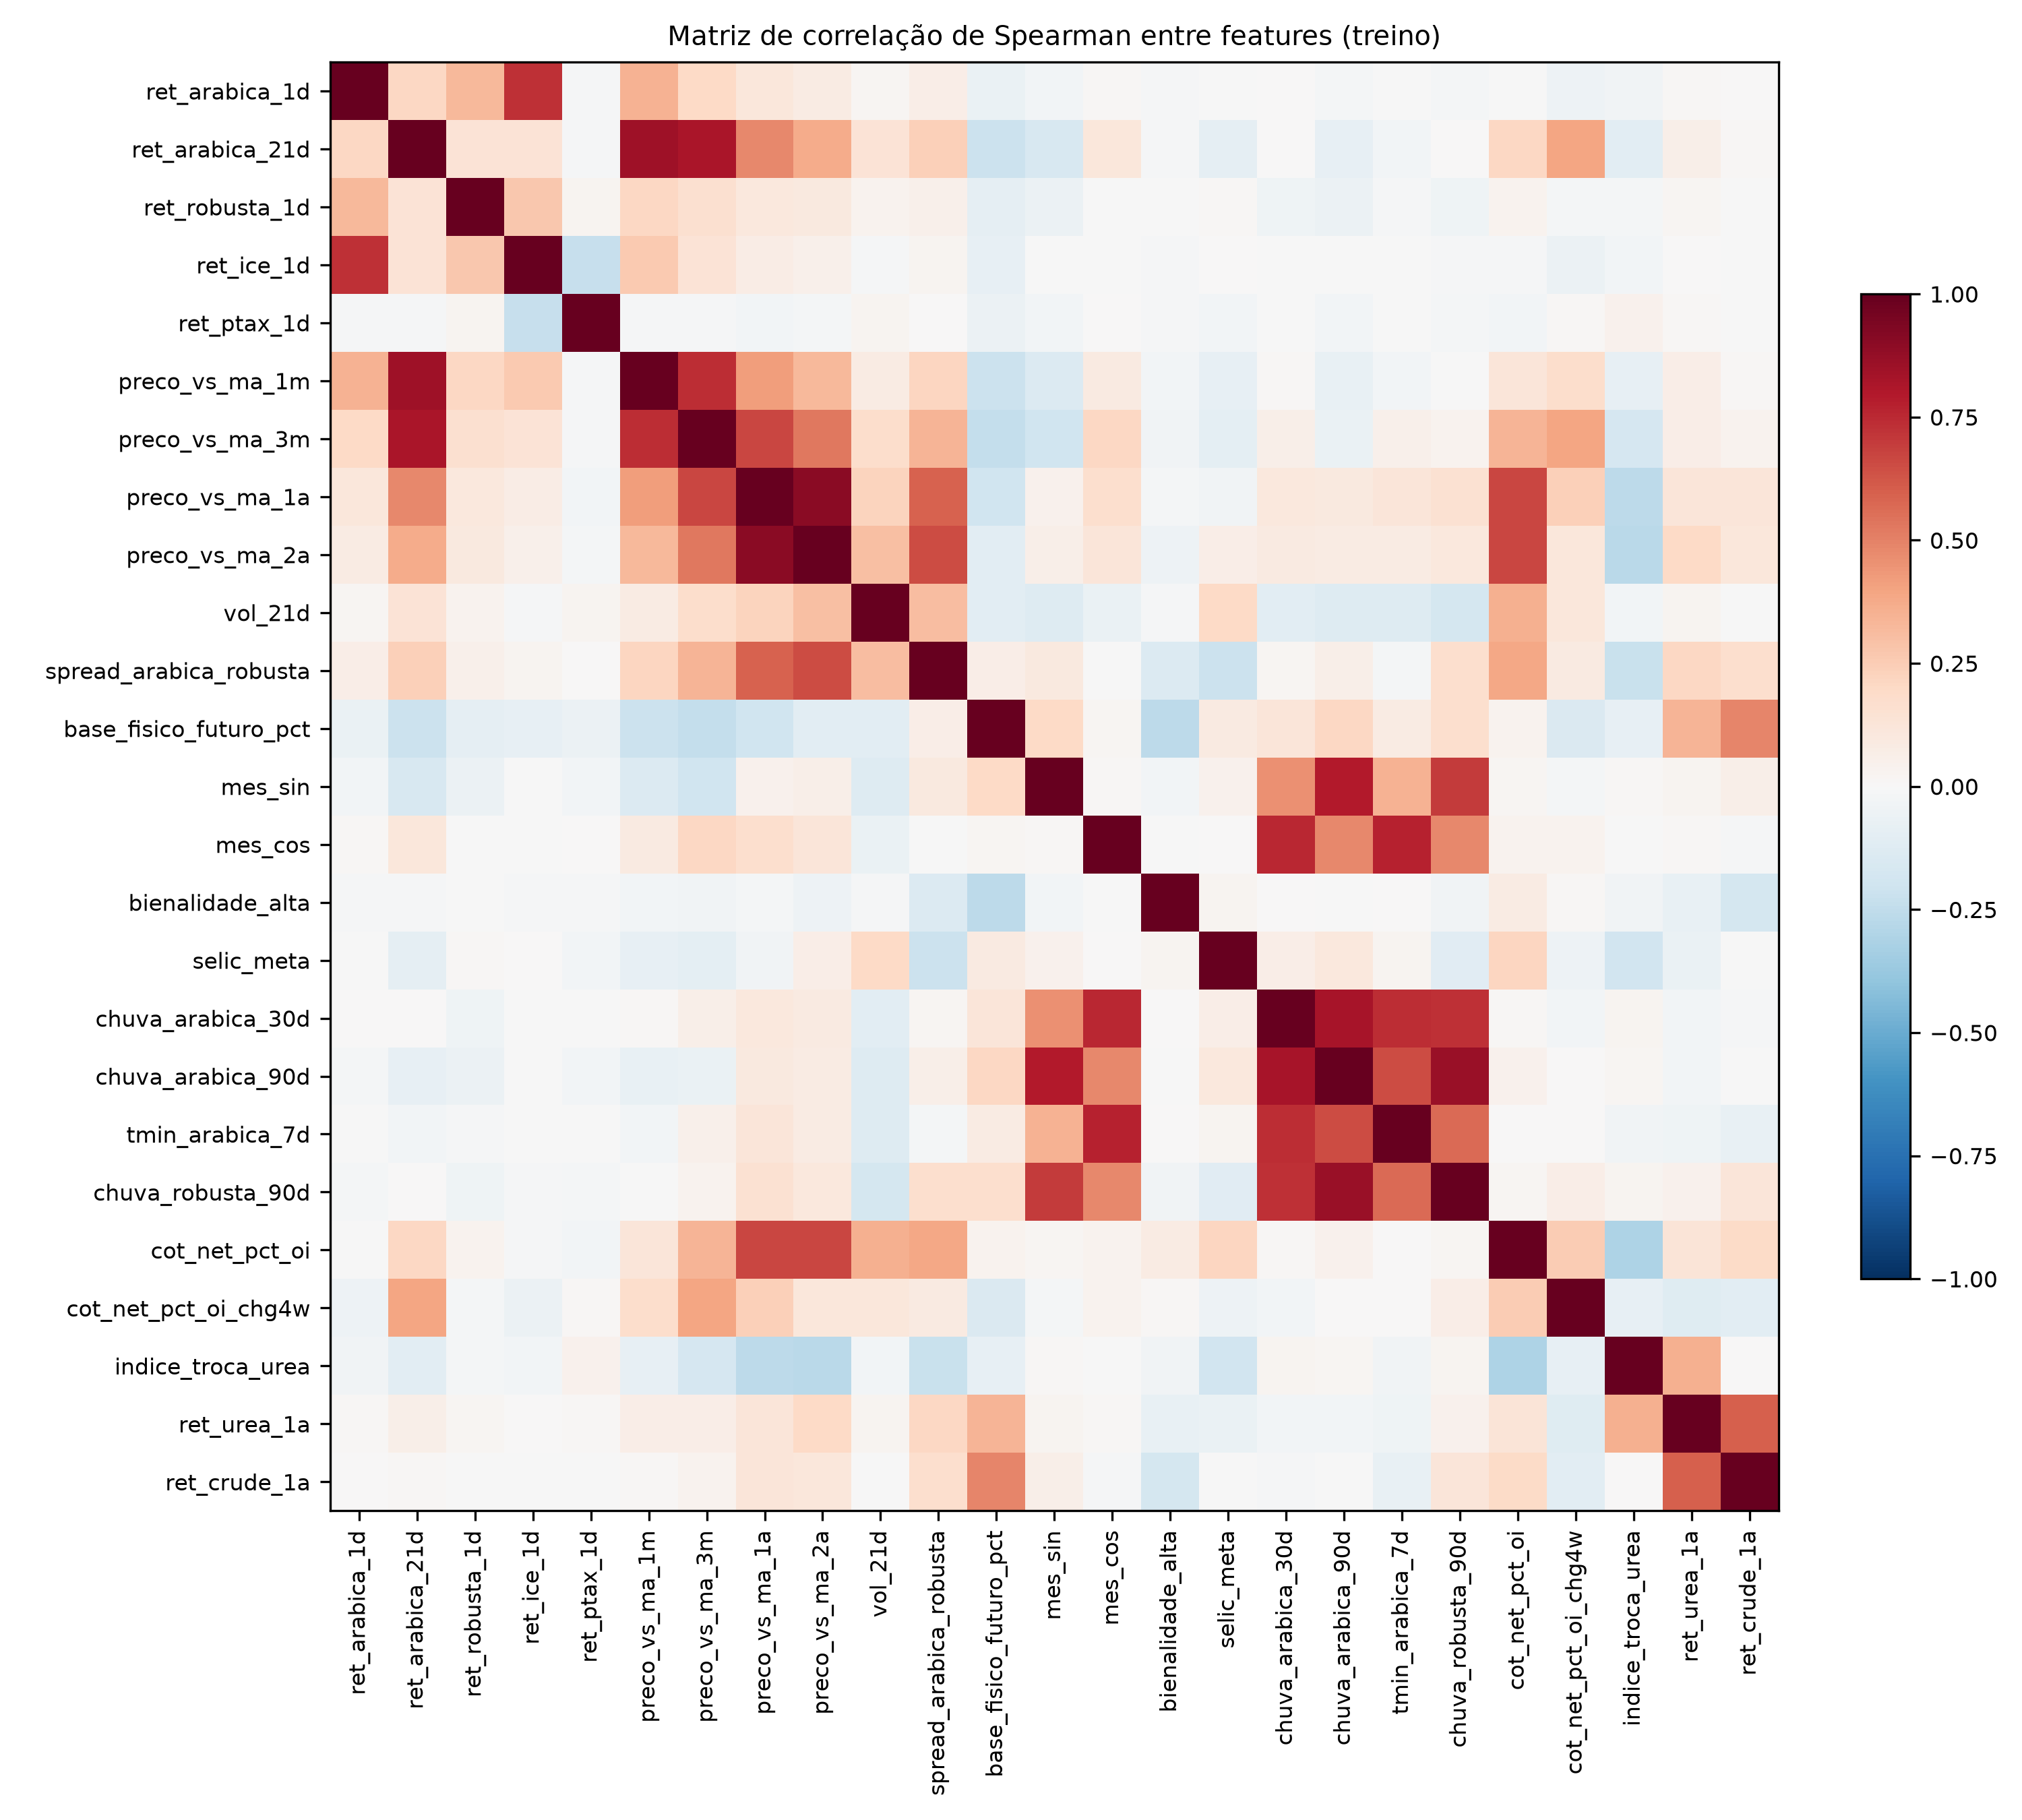
\includegraphics[width=0.95\textwidth]{imgs/11_matriz_corr_features.png}
	\fonte{Do autor (2026).}
\end{figure}

Três padrões orientaram as decisões seguintes. Primeiro, o sinal está nas variáveis de oferta, de base e de calendário, e cresce com o horizonte: o acumulado de chuva de 90 dias nas regiões de arábica tem correlação de $-0{,}37$ com o retorno de 63 dias, a base físico-futuro de $-0{,}34$ com o de 126 dias, o acumulado de 30 dias de $-0{,}31$ com o de 126 dias, a mínima de sete dias de $-0{,}26$ e a meta Selic de $-0{,}23$ no mesmo horizonte. O sinal negativo da chuva é o esperado: chuva abundante na floração melhora a expectativa da safra seguinte e o mercado a precifica para baixo. Segundo, as variáveis de curto prazo carregam pouco ou nenhum sinal: retornos diários, retorno de 21 dias, posição em relação às médias de um e três meses e volatilidade têm correlação inferior a $0{,}04$ em módulo em todos os horizontes. Terceiro, clima e calendário medem em parte a mesma coisa, a estação do ano: as correlações entre a codificação do mês e os acumulados de chuva e a mínima de temperatura ficam entre $0{,}7$ e $0{,}8$, e os acumulados de chuva de 90 dias das regiões de arábica e de robusta têm correlação $0{,}9$. Também são quase redundantes as razões com as médias de um e dois anos ($0{,}9$) e o retorno de 21 dias com a razão à média de um mês ($0{,}8$).

Nenhuma variável foi removida com base nessa análise. A rede recorrente tolera colinearidade entre entradas, o \textit{dropout} penaliza a dependência de uma única variável, e a contribuição de cada grupo é medida diretamente, por ablação e por importância por permutação, no \autoref{sec:resultados}. A colinearidade entre clima e calendário, porém, condiciona a leitura dessas medidas: ao remover um dos grupos, o outro pode compensá-lo em parte. A análise revelou ainda que o indicador de geada é constante igual a zero em toda a série, porque a reanálise ERA5 nunca registra temperatura mínima abaixo de 3\,$^{\circ}$C nos quatro pontos de grade escolhidos, nem mesmo em julho de 2021. A variável foi mantida entre as 26 entradas, onde é inerte após a normalização, e a consequência para a validade de construção é discutida no \autoref{sec:ameacas}.

\subsection{Partição temporal e normalização}

A partição é estritamente cronológica e usa o ano-safra, iniciado em julho, como unidade. O conjunto de teste cobre exatamente duas safras, porque a bienalidade define um ciclo de dois anos e uma única safra representaria apenas metade dele. A \autoref{tab:split} apresenta os cortes.

\begin{table}[htb]
	\centering
	\caption{Partição cronológica da base de dados.}\label{tab:split}
	\small
	\begin{tabular}{l L{3.3cm} L{2.6cm} r L{4.2cm}}
		\hline
		\textbf{Conjunto} & \textbf{Período} & \textbf{Safras} & \textbf{Amostras} & \textbf{Uso} \\ \hline
		Treino & 07/12/2005 a 30/06/2022 & 2005/06 a 2021/22 & 3\,940 & Pesos e normalizador \\
		Validação & 01/07/2022 a 30/06/2024 & 2022/23 e 2023/24 & 372 & Parada antecipada, dispersão residual, base sazonal \\
		Teste & 01/07/2024 a 31/08/2026 & 2024/25 e 2025/26 & 417 & \textit{Backtest} cego \\ \hline
	\end{tabular}
	\fonte{Do autor (2026).}
\end{table}

A janela de entrada de uma amostra pode cruzar a fronteira com o conjunto anterior, uma vez que se trata de histórico já conhecido na data da previsão. O alvo nunca cruza: as últimas 126 datas de cada conjunto são descartadas como origem de amostra, para que nenhum rótulo do treino seja calculado com preços da validação, nem rótulo da validação com preços do teste. Por esse motivo as amostras de validação terminam em dezembro de 2023 e as de teste em março de 2026.

A normalização usa um padronizador global ajustado exclusivamente no conjunto de treino e aplicado sem reajuste à validação e ao teste. A alternativa de normalizar em janelas deslizantes foi considerada e descartada porque as variáveis já são estacionárias por construção, o que torna o padronizador global suficiente e mais simples de auditar.

\section{Operacionalização da Ferramenta}\label{sec2:operacionalizacao}

O AgroVisible é organizado em dois módulos desacoplados. O módulo preditivo recebe a janela de variáveis e devolve a previsão central e a dispersão do log-retorno em cada horizonte. O módulo prescritivo recebe essa distribuição, os parâmetros econômicos do produtor e a curva de futuros, e devolve a política ótima. A interface entre os dois é apenas um vetor de médias e um vetor de desvios-padrão por horizonte, de forma que o módulo preditivo pode ser substituído por qualquer outro estimador sem alteração no motor de decisão.

\subsection{Módulo preditivo}

A rede é uma LSTM empilhada, implementada em Keras, com a arquitetura resumida no \autoref{qua:lstm}. Ela recebe uma janela de 63 dias úteis por 26 variáveis e produz três saídas treinadas em conjunto: o log-retorno em 21, 63 e 126 dias úteis,
\begin{equation}
	y_h(t) = \ln P(t+h) - \ln P(t), \qquad h \in \{21, 63, 126\},
\end{equation}
em que $P$ é o indicador CEPEA em R\$/sc. O preço projetado é reconstruído por $\hat{P}(t+h) = P(t)\,e^{\hat{y}_h(t)}$. A escolha de log-retornos como alvo, em vez do preço em nível, elimina a tendência da série e faz com que erros sejam comparáveis entre períodos de preço baixo e alto.

\begin{quadro}[htb]
	\centering
	\caption{Configuração do módulo preditivo.}\label{qua:lstm}
	\begin{tabular}{L{4cm} L{10cm}}
		\hline
		\textbf{Elemento} & \textbf{Configuração} \\ \hline
		Entrada & Janela de 63 dias úteis $\times$ 26 variáveis \\
		Camadas & LSTM(32, sequências) $\to$ Dropout 0,4 $\to$ LSTM(16) $\to$ Dropout 0,4 $\to$ Dense(32, ReLU) $\to$ Dense(3, linear) \\
		Saídas & Log-retorno em 21, 63 e 126 dias úteis \\
		Função de perda & Erro quadrático médio sobre os log-retornos \\
		Otimizador & Adam, taxa inicial $10^{-3}$, redução por patamar (fator 0,5, paciência 7) \\
		Treinamento & Até 100 épocas, lote 32, parada antecipada na perda de validação (paciência 15, restaura os melhores pesos); o modelo final parou na época 26 \\
		Seleção & Unidades e \textit{dropout} escolhidos por busca no conjunto de validação (\autoref{sec3:busca-hp}); janela, lote, taxa e paciências fixados a priori \\
		Reprodutibilidade & Semente 42; execução em CPU \\ \hline
	\end{tabular}
	\fonte{Do autor (2026).}
\end{quadro}

Além da previsão central, o módulo estima a incerteza da previsão pelo desvio-padrão dos resíduos $\hat{y}_h - y_h$ no conjunto de validação, um valor por horizonte. Esse desvio é o único canal pelo qual a qualidade da previsão chega ao motor de decisão: quanto maior o erro histórico da rede em um horizonte, mais largo é o cone de preços que o motor considera nesse horizonte.

\subsection{Busca de hiperparâmetros}\label{sec3:busca-hp}

A configuração inicial do módulo preditivo foi fixada a priori, antes de qualquer experimento: 64 unidades na primeira camada recorrente e 32 na segunda, \textit{dropout} 0,2, janela de 63 dias úteis, escolhida por cobrir um trimestre, igual ao horizonte intermediário, lote 32 e taxa de aprendizado $10^{-3}$. Para verificar se essa capacidade era adequada a uma amostra de 3\,940 janelas de treino, foi conduzida uma busca em duas etapas, sobre o conjunto de validação e sem uso do conjunto de teste para escolher.

Na primeira etapa, uma grade de doze configurações variou um fator por vez a partir da configuração inicial: unidades (32 e 128), \textit{dropout} (0 e 0,4), janela (21 e 126 dias), taxa de aprendizado ($3 \times 10^{-4}$ e $3 \times 10^{-3}$) e lote (64), além de duas candidatas enxutas com 32 unidades e \textit{dropout} 0,4, uma com janela de 63 e outra de 126 dias. Cada configuração foi treinada uma única vez, com semente 42 e o mesmo critério de parada antecipada, e comparada pelo RMSE em cada horizonte e pela média dos três horizontes na validação. O RMSE de treino foi registrado como indicador de sobreajuste: uma configuração que erra muito menos no treino do que na validação está memorizando a amostra.

Na segunda etapa, as três configurações mais promissoras, a inicial e as duas de 32 unidades com janela de 63 dias, foram retreinadas com cinco sementes (42 a 46) e avaliadas na validação e no teste, reportando média e desvio-padrão entre sementes ao lado dos métodos de referência. A escolha do modelo final foi feita pela média de validação; as métricas de teste dessa etapa servem apenas para confirmar que a ordem entre as candidatas não é um artefato do conjunto de validação. Os resultados da busca estão na \autoref{sec2:res-hp}, e a implicação de ter selecionado a arquitetura na validação é tratada como ameaça à validade interna no \autoref{sec:ameacas}.

\subsection{Módulo prescritivo}

O problema de comercialização é formulado como um processo de decisão de Markov de horizonte finito \cite{Puterman1994}, resolvido por indução retroativa sobre a equação de Bellman \cite{Bellman1957}.

\paragraph{Tempo e estado.} O tempo avança em passos mensais $k = 0, 1, \ldots, K$, com $K = 6$ (126 dias úteis), que é o horizonte máximo de previsão da rede. O estado é o par $(k, x)$, em que $x = \ln P$ é o logaritmo do preço físico em R\$/sc, discretizado em uma grade de 121 pontos centrada no preço da data de decisão.

\paragraph{Transição.} O log-preço evolui por incrementos gaussianos cuja média e variância vêm do módulo preditivo:
\begin{equation}
	x_{k+1} = x_k + \Delta\mu_k + \varepsilon_k, \qquad \varepsilon_k \sim \mathcal{N}(0, \Delta\sigma_k^2).
\end{equation}
A previsão central e o desvio residual dos três horizontes são interpolados linearmente para os sete passos mensais; a variância acumulada é forçada a ser não decrescente. A transição entre grades consecutivas é uma matriz gaussiana discretizada e normalizada por linha. Não há amostragem de cenários: a indução retroativa integra sobre toda a distribuição em cada passo.

\paragraph{Ações.} Em cada estado o produtor escolhe entre três ações:
\begin{alineas}
	\item \textbf{vender}: recebe $P_k (1-q)^k$ por saca, em que $q$ é a quebra técnica mensal, e encerra o processo;
	\item \textbf{armazenar}: paga o custo de armazenagem $c_{\text{arm}}$ do mês e segue exposto ao preço;
	\item \textbf{armazenar com \textit{hedge}} até o vencimento $m > k$: vende o contrato futuro de vencimento $m$ e armazena até lá, recebendo o preço travado $F_{k,m}(1 + b_m) - c_{\text{op}}$, sujeito apenas ao risco de base, em que $b_m$ é a base sazonal esperada no mês $m$ e $c_{\text{op}}$ o custo operacional de bolsa.
\end{alineas}

\paragraph{Função de valor.} A recompensa é a receita líquida por saca trazida a valor presente na data da decisão. O fator de desconto mensal deriva da meta Selic vigente, $\delta = (1 + i_{\text{Selic}})^{-1/12}$, e representa o custo de oportunidade do capital imobilizado no estoque. A função de valor é
\begin{equation}
	V_K(x) = P(x)\,(1-q)^K,
\end{equation}
\begin{equation}
	V_k(x) = \max\Big\{\, P(x)(1-q)^k,\;\; -c_{\text{arm}} + \delta\,\mathrm{CE}\big[V_{k+1}\big],\;\; \max_{m > k} H_{k,m}(x) \Big\}, \quad k < K,
	\label{eq:bellman}
\end{equation}
em que $H_{k,m}$ é o valor presente do \textit{hedge} até $m$ e $\mathrm{CE}[\cdot] = \mathbb{E}[\cdot] - \lambda\,\mathrm{DP}[\cdot]$ é o equivalente certo, com $\lambda \geq 0$ o parâmetro de aversão a risco do produtor. Com $\lambda = 0$ o produtor é neutro a risco e maximiza a receita esperada.

O custo operacional efetivo (COE) entra no motor como piso econômico da comercialização. Como o COE é um custo já incorrido na data da decisão, ele não altera a comparação marginal entre vender e armazenar em um dado estado; seu papel é outro: vender abaixo do COE configura descapitalização da empresa rural \cite{AgroSafety2026}, e a ferramenta sinaliza ao produtor a margem sobre o COE em cada nó do grafo e classifica o resultado esperado de cada ação nas faixas de lucro supernormal, lucro normal, resíduo financeiro, descapitalização ou falência, conforme a relação entre a receita esperada e as camadas de custo COE, COT e custo total médio. Adicionalmente, o motor oferece uma restrição opcional, desligada por padrão, que só permite a ação de vender em nós com preço igual ou superior a COE$\times$(1 + m), com m uma margem mínima configurável, enquanto houver horizonte; no último período a venda é forçada. O COE por safra é lido da série histórica de custos de produção da CONAB para o café arábica em Guaxupé, Minas Gerais, com a correspondência COE = custo variável, COT = custo operacional e custo total conforme a nomenclatura da planilha.

\paragraph{Parâmetros econômicos.} A \autoref{tab:parametros} lista os valores padrão. A armazenagem e a quebra técnica são referências de mercado de armazéns gerais; a Selic é lida da série do Banco Central na data da decisão; o custo operacional de bolsa segue material de capacitação em gestão de risco agrícola.

\begin{table}[htb]
	\centering
	\caption{Parâmetros econômicos padrão do módulo prescritivo.}\label{tab:parametros}
	\small
	\begin{tabular}{L{5cm} L{4.6cm} L{4.2cm}}
		\hline
		\textbf{Parâmetro} & \textbf{Valor padrão} & \textbf{Origem} \\ \hline
		Armazenagem $c_{\text{arm}}$ & 2,50 R\$/sc/mês & Referência de armazém geral \\
		Quebra técnica $q$ & 0,2 \%/mês & Referência de mercado \\
		Taxa de desconto & 10\,\% a.a. (Selic vigente na sensibilidade) & BCB, série 432 \\
		Custo operacional de bolsa $c_{\text{op}}$ & 10 R\$/sc & Material de capacitação \\
		COE por safra & 766 a 876 R\$/sc & CONAB, Guaxupé, MG \\
		Aversão a risco $\lambda$ & 0 & Parâmetro do usuário \\ \hline
	\end{tabular}
	\fonte{Do autor (2026).}
\end{table}

\paragraph{Grafo de decisão.} O objeto que o motor resolve é uma cadeia de Markov em camadas: sete camadas temporais com 121 nós de preço cada, e arestas de cada nó para todos os nós da camada seguinte, ponderadas pela transição gaussiana. A indução retroativa percorre esse grafo direcionado acíclico da última camada para a primeira, e o resultado é a ação ótima em cada nó, o gatilho de preço a partir do qual vender é ótimo em cada mês, e a distribuição de probabilidade do mês de venda. Para fins de apresentação ao produtor, uma árvore reduzida com três ramos por mês (quantis 10, 50 e 90 do cone de preços) é anotada com as ações lidas da política completa; essa árvore ilustra a política, mas não participa do cálculo.

\paragraph{Base e \textit{hedge}.} A base é definida em percentual do futuro convertido, $b = (P - F_{\text{R\$}}) / F_{\text{R\$}}$, em que $F_{\text{R\$}}$ é o \textit{Coffee C} convertido de centavos de dólar por libra-peso para reais por saca de 60 kg pela PTAX do dia. A modelagem em percentual, e não em reais, decorre da observação de que a base em reais escala com o nível de preço. A base esperada por mês do ano e o risco de base por horizonte (desvio-padrão da variação da base) são estimados de 2015 até o fim do conjunto de treino. O contrato ICE convertido é usado como \textit{proxy} do contrato ICF da B3, cuja série histórica não está disponível publicamente.

\paragraph{Operação em política rolante.} Em uso corrente, o sistema é executado a cada data de decisão com a janela de 63 dias úteis encerrada naquela data; a rede recebe apenas dados já observados e publicados até ela, respeitando as datas de disponibilidade descritas na \autoref{sec2:pipeline}. A previsão nova substitui a anterior, o horizonte de seis meses é recontado a partir da nova data e a política é resolvida de novo. Uma saca que foi armazenada no mês anterior é, portanto, reavaliada com a informação mais recente e vendida assim que a ação ótima do novo estado for vender, mesmo que a política do mês anterior previsse mantê-la por mais tempo. O produtor recebe, a cada mês, a ação do dia, o gatilho de venda por mês futuro e a distribuição de probabilidade do mês de venda. É esse mecanismo rolante que o \textit{backtest} e a simulação por safra reproduzem. Neste estudo a rede foi treinada uma única vez, com dados até junho de 2022, e não é retreinada entre decisões; a periodicidade de retreino em operação é uma decisão de implantação, discutida no \autoref{sec:discussao}.

\section{Protocolo de Avaliação}\label{sec2:protocolo}

\subsection{Avaliação preditiva (RQ1)}

A acurácia é medida no conjunto de validação e no conjunto de teste, por horizonte, com RMSE e MAE no espaço do log-retorno e MAPE no preço reconstruído, além da acurácia direcional (proporção de previsões com o sinal correto). Os métodos de referência são:
\begin{alineas}
	\item \textbf{passeio aleatório}: retorno previsto igual a zero em todos os horizontes;
	\item \textbf{curva de futuros com base sazonal}: retorno implícito $\ln\big[F_t\,(1 + b_{t+h}) / P_t\big]$, em que $F_t$ é o futuro convertido e $b_{t+h}$ a base sazonal esperada no mês de destino;
	\item \textbf{ARIMA} sobre o log-preço diário, com ordem $(p,d,q)$, $p,q \in \{0,1,2\}$, selecionada por AIC no conjunto de treino; parâmetros fixos, previsão recursiva a partir de cada data.
\end{alineas}

A seleção da arquitetura segue o protocolo da \autoref{sec3:busca-hp}: grade de doze configurações com semente única e verificação das candidatas com cinco sementes. Como referência para a variabilidade de treino, o modelo final é treinado com cinco sementes distintas, e toda diferença entre modelos menor que o desvio-padrão entre sementes é tratada como empate.

A contribuição das variáveis exógenas é medida por três instrumentos complementares. A correlação de Spearman com o alvo, calculada antes do treinamento (\autoref{sec3:eda}), indica onde há sinal nos dados. A importância por permutação mede, no modelo final treinado, o aumento do RMSE de validação quando os valores de uma variável são embaralhados dentro da janela de entrada, na média de três permutações; ela indica de quais variáveis a rede efetivamente depende. A ablação, por fim, retreina a rede com a mesma configuração removendo, um por vez, cada um de seis grupos de variáveis (retornos e médias móveis; mercado; calendário e Selic; clima; fundos; insumos), com três sementes por configuração, e registra a variação relativa do RMSE médio por horizonte; ela indica o que se perde quando o grupo não está disponível.

\subsection{Avaliação prescritiva (RQ2)}

O \textit{backtest} simula um produtor que, em cada data de decisão, dispõe de uma saca colhida e deve decidir o que fazer com ela ao longo dos seis meses seguintes. As datas de decisão são mensais, de 1º de julho de 2024 a 3 de fevereiro de 2026, totalizando 20 decisões distribuídas em duas safras. Em cada data o motor é resolvido com a previsão e a Selic daquela data, sem acesso a qualquer informação posterior, e a política é executada contra os preços efetivamente observados. A receita de cada estratégia é a receita líquida por saca em valor presente na data da decisão, com a mesma contabilidade de armazenagem, quebra e desconto para todas.

As estratégias comparadas são:
\begin{alineas}
	\item \textbf{venda imediata}: vende na data da decisão e aplica o valor à taxa de desconto até o fim do horizonte. Como todas as receitas são trazidas a valor presente pela mesma taxa, isso equivale a comparar cada estratégia com a alternativa de vender hoje e investir o resultado à Selic;
	\item \textbf{venda parcelada}: vende um sexto da saca em cada um dos seis meses;
	\item \textbf{média móvel de três meses}: vende quando o preço cruza acima da média móvel de 63 dias, ou no fim do horizonte;
	\item \textbf{meta de margem sobre o COE}: vende quando o preço alcança 130 \% do COE, ou no fim do horizonte;
	\item \textbf{\textit{hedge} de seis meses}: vende o futuro na data da decisão e entrega no fim do horizonte;
	\item \textbf{AgroVisible}: executa a política ótima resolvida pela \autoref{eq:bellman};
	\item \textbf{oráculo}: vende no melhor mês do horizonte com conhecimento perfeito do futuro; é o limite superior, não uma estratégia viável.
\end{alineas}

As duas primeiras são as heurísticas nomeadas na RQ2. As demais foram acrescentadas por serem praticadas por produtores e cooperativas e por isolarem componentes específicos do AgroVisible: a média móvel testa uma regra técnica simples; a meta de margem testa uma regra de custo; o \textit{hedge} fixo testa o instrumento de proteção isoladamente. O oráculo permite expressar o ganho de cada estratégia como fração do ganho máximo disponível.

O mesmo protocolo é aplicado às 18 datas mensais do período de validação, de julho de 2022 a dezembro de 2023, que contém regime de queda de preços, ampliando a amostra para 38 decisões em quatro safras. Nesse período a dispersão residual e a parada antecipada da rede foram calibradas com os próprios dados, o que é declarado como viés favorável leve ao interpretar os resultados. A significância das diferenças de receita é avaliada por diferença pareada por data, com intervalo de confiança de 95\,\% por \textit{bootstrap} de 10\,000 reamostragens e teste de Wilcoxon pareado.

\paragraph{Simulação por safra.} O \textit{backtest} mensal avalia vinte decisões independentes, cada uma com uma saca recém-colhida, o que mede a qualidade média da política, mas não reproduz a situação do produtor, que colhe uma vez por ano. Por isso o mesmo motor é avaliado em uma segunda forma: uma saca colhida no primeiro dia útil de julho de cada ano-safra, de 2022 a 2025, com até doze meses para ser vendida. A política é rolante, como descrito na \autoref{sec2:operacionalizacao}: a cada mês o motor é resolvido de novo com a previsão daquela data e o prazo restante, e a saca é vendida no primeiro mês em que a ação ótima for vender. Como o horizonte de doze meses excede o alcance de 126 dias da rede, além desse ponto a deriva prevista é mantida no último valor e a incerteza cresce com a raiz do tempo, como em um passeio aleatório, extrapolação conservadora que só afeta os meses finais de uma trajetória que é reavaliada mensalmente. As mesmas estratégias de referência são simuladas no horizonte de doze meses e a receita é expressa em valor presente na data da colheita. As safras 2024/25 e 2025/26 são cegas; 2022/23 e 2023/24 pertencem ao período de validação, com o viés já declarado.

\subsection{Análise de sensibilidade (RQ3)}

A sensibilidade é avaliada repetindo o \textit{backtest} completo sob uma grade de parâmetros e registrando a receita líquida média e a frequência de decisões de armazenar. A grade cobre a aversão a risco ($\lambda \in \{0; 0{,}25; 0{,}5; 1\}$), o custo de armazenagem ($\{1{,}5; 2{,}5; 5{,}0\}$ R\$/sc/mês), a taxa de desconto (8, 10, 12, 13,25 e 15\,\% a.a., além da Selic vigente em cada data) e o choque de base (deslocamento de $\pm 5$ pontos percentuais na base esperada e duplicação do risco de base). O caso base adota taxa de desconto de 10\,\% a.a., valor próximo à média da Selic na amostra.

\subsection{Ambiente de execução}

Todos os experimentos foram executados em Python 3.13, com TensorFlow 2.21 e Keras 3.15 para a rede neural, NumPy 2.5 e SciPy 1.18 para o motor de decisão, pandas 3.0 para o alinhamento dos dados, scikit-learn 1.9 para a normalização e statsmodels 0.15 para o ARIMA, em um computador pessoal com Windows 11, em CPU, sem aceleração por GPU, e com semente fixa. O código está organizado em cinco cadernos numerados (coleta, variáveis, previsão, decisão e simulação por safra) e em módulos reutilizáveis, de modo que cada tabela e figura dos capítulos seguintes pode ser regenerada a partir dos dados brutos. O código, os dados e os resultados intermediários estão versionados em um repositório Git.
